
\documentclass[a4paper]{report}

\usepackage{jheppub}
\pagestyle{myplain}

\usepackage{amsmath}
\usepackage{algorithmic}
\usepackage{array}
\usepackage{siunitx}
\usepackage{url}
\usepackage{hyperref}
% \usepackage{subcaption}
\usepackage{lipsum}

\begin{document}

\title{Simulating the Measurement of the\\Electron Beam Emittance at AWAKE}
\author{Patrick~Chin,}
\author{Emma~Simpson~Dore,}
\author{Lawrence~Deacon,}
\author{Fearghus~Keeble,}
\author{Simon~Jolly,}
\author{and Matthew~Wing}
\emailAdd{p.ch@live.co.uk}
\emailAdd{emma.dore.13@ucl.ac.uk}
\affiliation{Department of Physics and Astronomy, University College London,\\
	Gower Street, London, England}
\collaboration{The AWAKE Collaboration}

\abstract{
	In preparation for the experiments at AWAKE, simulations were used to
	determine to what precision the spectrometer is to be able to measure the
	emittance of the accelerated electron beam. A range of experimental
	parameters, including bunch size, energy, energy spread, emittance were
	tested and the degree to which these parameters effect the measurement of
	the emittance were determined. Systematic errors arising from the discrete
	pixels on the screen were found to increase the measurement emittance by
	\SI{1e-8}{\meter\radian}.
}

\keywords{plasma wakefield, spectrometer, emittance, electron beam, simulation}


\maketitle
% \tableofcontents
\newpage


\section{Introduction}

Advancements in quantum and particle physics are primarily driven by
experimental observations which can verify or refute previous hypotheses, or
can provide data from which new hypotheses can be drawn. 
% This allows us to have a deeper understanding of the universe around us.
Particle colliders are a main source of observational data at the quantum
scale, and can create millions of collision events every second.

%TODO
% Improvements to these colliders come in the form of increasing the luminosity
% of the beam.  beam energy come largely in the form of increasing the energy
% of the colliding particle beams.

Proton--proton beam energies at the Large Hadron Collider (LHC) have recently
reached energies of \SI{13}{\tera\electronvolt} \cite{o2015first}, whereas
lepton--lepton colliders have yet to reach the \si{\tera\electronvolt} energy
scale. The largest of which, the Large Electron-Proton Collider (LEP), was
closed down to make way for the LHC in \num{2000} after having reached a
maximum energy of \SI{209}{\giga\electronvolt} \cite{Barate2003sz}.

\begin{itemize}
	\item reasons why lepton collisions are cleaner than protons
	\item drawbacks of circular accelerator synchrotron radiation at LEP
		\cite{Brandt2000xk}
	\item ICL and CLIC proposed linear RF accelerators ten times larger
		than SLAC
\end{itemize}

% however protons are
% not fundamental particles meaning the energy of each constituent particle is
% less than that of the beam. Leptons however, are fundamental point-like
% particles meaning their centre-of-mass energy can be determined to a higher
% precision and also the collision environment will be much cleaner.

% Looking at current accelerators, circular electron or positron accelerators are
% not possible at these energies unless the accelerator reaches the
% \SI{100}{\kilo\meter} scale as electrons at this energy approach the speed of
% light and since they are accelerating in a circle they will radiate large
% amounts of their energy.
% % \cite{sokolov1966synchrotron}
% An accelerator at the \SI{100}{\kilo\meter} scale is
% impractical due to geographical and financial limitations.  Similar problems
% also arise in linear colliders where current radio-frequency (RF) cavities in a
% linear collider will have to be tens of kilometres in length to reach the
% \si{\tera\electronvolt} scale, this is with current acceleration gradients of
% up to \SI{100}{\mega\volt\per\meter}.  This urges the development of a new
% methods for the acceleration of particles.

The CLIC and ICL are promising proposals for lepton--lepton colliders to reach
the \si{\tera\electronvolt} scale, however

continuing to increase the energy of colliding beams allows for an increasing
number of interactions to be observed.

\section{Proton Driven Plasma Wakefield Acceleration}

Current radio-frequency (RF) accelerator technology is limited to an
electromagnetic gradient of about \SI{100}{\mega\electronvolt\per\meter} due to
RF beakdown.  The ability of plasma to sustain very large 

The concept of accelerating particles in plasma was promising as plasma is able
to sustain large electric fields.  The idea being that energy can be
transferred to a group of charged particles by injecting them into the plasma
wakefield that follows a high energy laser pulse or proton bunch, using the
plasma as an energy transfer medium.  The witness bunch is then accelerated by
the high electromagnetic gradient.

\section{AWAKE}

\subsection{Self-modulation instability}

The first challenge in the development of this accelerator was getting the
length of the proton driver bunch small enough so that resonance occurs with
the electrons in the plasma.  Typical proton bunches, i.e. those produced by
the CERN Super Proton Synchrotron (SPS), have lengths of \(\sim
\SI{10}{\centi\meter}\) which cannot directly create strong plasma waves at the
required wavelength in the \si{\milli\meter} scale as the Fourier component of
the proton beam at the plasma frequency is negligible.
Simulations~\cite{kumar2010self} on the compression of these bunches show that
reducing the longitudinal phase volume blows up the transverse phase volume.
An alternative method would be to split up the proton bunch into a number of
micro-bunches to be simultaneously decelerated.

An instability between the beam and the plasma arises from the mutual
amplification of the rippling of the beam radius and the plasma wave. This
instability tends to destroy the plasma wave as the amplification focuses and
defocuses selected slices of the beam.  This problem was solved by seeding the
self-modulated instability (SMI) with a short electron bunch
\cite{lotov2013natural}, a laser pulse \cite{siemon2013laser} or a sharp cut in
the bunch profile\cite{kumar2010self}. This will promote a single mode and
suppress other modes, including the strongest competing modes, the hosing modes
\cite{vieira2014hosing} and produce well-separated micro-bunches.

\subsection{Uniform-density plasma cell}

The plasma wavelength is \(\lambda_{pe} \approx \SI{1.26}{\milli\meter}\)
meaning that the \SI{10}{\centi\meter} proton bunch will have to be split into
\(\sim 100\) micro-bunches in order to be able to drive the wake.  Each
micro-bunch contributes to the wakefield, and only if the plasma density is
uniform will the contribution of each bunch be coherent. Incoherence will cause
the electron bunches to arrive at the wrong phase in the plasma oscillation. An
increase in the plasma density will shorten the plasma wavelength causing the
electron bunch to crest plasma wave it was riding and fall into the defocusing
phase of the plasma wave as shown in Fig \ref{fig:phases}(a). A decrease
in the plasma density will increase the plasma wavelength causing the plasma
wave to fall further behind the electron bunch meaning the electron bunch to
fall into the trough of the plasma wave resulting in a deceleration of the
electron beam \ref{fig:phases}(c). The electron beam must be in the
region of length \(\lambda_{pe}/4\) between the defocusing and decelerating
phases of the plasma wave.
% These effects are significantly larger for the electrons as protons have
% large longitudinal momentum.

\begin{figure}[tb]
	\centering
	\begin{subfigure}{\linewidth}
		\centering
		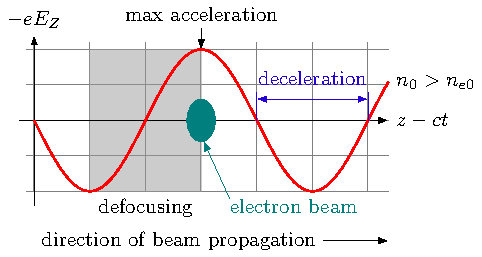
\includegraphics[width=0.9\linewidth]{figures/phases-a.pdf}
		\caption{asdkfjasdlfj sdk dfs f}
	\end{subfigure}
	\begin{subfigure}{\linewidth}
		\centering
		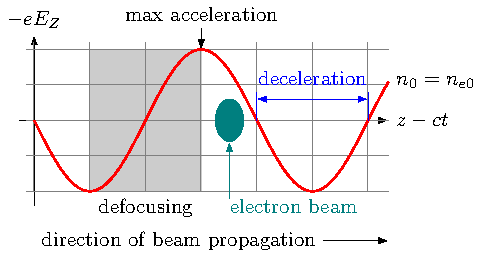
\includegraphics[width=0.9\linewidth]{figures/phases-b.pdf}
		\caption{asdkfjasdlfj sdk dfs f}
	\end{subfigure}
	\begin{subfigure}{\linewidth}
		\centering
		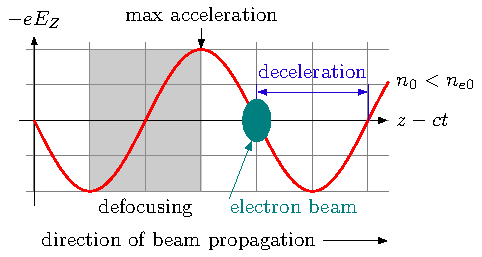
\includegraphics[width=0.9\linewidth]{figures/phases-c.pdf}
		\caption{asdkfjasdlfj sdk dfs f}
	\end{subfigure}
	\caption{
		Phasing of the electron bunch for increased density (a) correct density
		(b) and decreased density (c). \cite{wiedemann2007particle}
	}
	\label{fig:phases}
\end{figure}

This requirement of the plasma limits the plasma selection to being uniform
rubidium vapor, ionised by a co-propagating laser pulse \cite{oz2014novel,
oz2014bja}.  Rubidium was chosen due to it's low ionization potential and heavy
atomic mass.  A heavy element is required to minimize the movement of the
plasma's nuclei which causes adverse effects on the plasma's behaviour
\cite{vieira2012nj, vieira2014bqa}. The Rubiduim vapor is kept in thermodynamic
equilibrium at a constant temperature and volume.

\subsection{Injection of the witness beam}

Due to SMI, the shape of the drive beam changes in the plasma and for the first
four meters, the difference between the phase velocity of the wakefield and the
proton beam velocity is quite large and this will effect the electron beam in
the same manner as having a non uniform plasma, detailed above. To avoid this
problem it was suggested that the electrons could be injected into the plasma
after SMI had fully developed. The design of the injection method arrived at
passing the electron beam through a narrow vacuum tube separated from the
plasma by a thin foil. Then after \(\sim \SI{4}{\meter}\) the electrons will be
directed into the wakefield close close behind the proton driving beam.

\subsection{AWAKE}

The aim of this experiment is to provide a proof of concept for proton driven
plasma wakefield acceleration.  An overview of the experiment is as follows:

The SPS will provide the \SI{400}{\giga\electronvolt} proton driver beam with a
bunch length of \(\sigma_z = \SI{12}{\centi\meter}\) and an intensity of \(\sim
3\times 10^{11}\) protons/bunch. This will travel down the \SI{750}{\meter}
long CNGS transfer line and be focused to \(\sigma_{x,y} =
\SI{200}{\micro\meter}\) and enter a \SI{10}{\meter} long Rubiduim vapor plasma
cell with an adjustable density at the \(10^{14}\) to \(10^{15}\)
electrons/\si{\per\centi\meter} scale.

The proton driver will self modulate at the plasma wavelength \(\lambda_{pe}\)
after being seeded by a high powered \(\approx \SI{4.5}{\tera\watt}\) laser
pulse that is co-axial and co-propagating with the proton driver beam. This
laser also serves the purpose of ionising the Rubidium vapor. These two beams
need to be synchronous to within \SI{100}{\pico\second} and the focal point of
the proton beam is required to be \(\le\SI{100}{\micro\meter}\) and
\(\le\SI{15}{\micro\radian}\) so they are co-axial for the full length of the
plasma cell.

The electron witness beam will be created via photo-emission by an illuminating
cathode electron source and accelerated by a 2.5 cell RF-gun and a meter long
booster at \SI{3}{\giga\hertz}.

%TODO injection

\section{Project outline}

% \lipsum[3-10]

The development of this experiment has been heavily simulation driven.
Simulation code developed specifically for the simulation of the plasma to be
able to resolve for time scales of \(\omega_p^{-1}\), (where \(\omega\) is the
frequency of the plasma wave) and length scales of down to \(c/\omega_p\), as
existing codes were not tuned to resolve at these scales.  Different simulation
softwares are tuned to be used for different sections of the AWAKE experiment.

% I will be working on simulating the electron spectrometer using
% BSDIM~\cite{agapov2009bdsim}, simulation software in active development,
% designed to simulate and track particle beams passing through accelerators and
% detectors. It is built on top of the Geant4
% toolkit~\cite{agostinelli2003geant4} for the simulation of particles through
% matter, which also provides the graphical user interface for a visualisation of
% the simulation.  Event data is stored using ROOT~\cite{antcheva2011root}, an
% advanced statistical analysis and visualisation framework designed to work for
% petabyte scale data storage.

% More specifically, I will initially be looking at calculating the emittance of
% the accelerated electron beam using data from simulated accelerated electron
% beams.  Recent simulations of the spectrometer used an idealised electron beam
% \cite{deacon2016qjq} and I will be continuing this line of investigation.  The
% electron beam profile and other properties immediately after it leaves the
% plasma cell will be provided by separate simulations using LCODE.  This data is
% used as input for the BDSIM simulation where we will simulate the beam passing
% through dual focusing quadrupoles in both the horizontal and vertical planes.
% The simulation will be able to provide all the raw data about the final state
% of the electron beam, however, in reality we will not be able to simply query
% the beam properties. The measurement of the energy spectrum will be carried out
% by using a magnetic dipole downstream of the dual quadrupoles, and observing
% the horizontal spread of the electron beam on a screen. This screen will also
% be sumulated with BDSIM taking into account the screen resolution and detection
% rates.

% I will also be working on the modeling and simulation of the background
% radiation from the plasma cell and other sources using real world data to help
% build an accurate model.  All of these simultions along with real data will
% help in finding optimal parameters for each component of the spectrometer,
% including the strength of the quadrupoles and the dipole, the lens parameters
% of the camera and the properties of the screen.



\chapter{Project outline}

\lipsum[3-56]

The development of this experiment has been heavily simulation driven.
Simulation code developed specifically for the simulation of the plasma to be
able to resolve for time scales of \(\omega_p^{-1}\), (where \(\omega\) is the
frequency of the plasma wave) and length scales of down to \(c/\omega_p\), as
existing codes were not tuned to resolve at these scales.  Different simulation
softwares are tuned to be used for different sections of the AWAKE experiment.

% I will be working on simulating the electron spectrometer using
% BSDIM~\cite{agapov2009bdsim}, simulation software in active development,
% designed to simulate and track particle beams passing through accelerators and
% detectors. It is built on top of the Geant4
% toolkit~\cite{agostinelli2003geant4} for the simulation of particles through
% matter, which also provides the graphical user interface for a visualisation of
% the simulation.  Event data is stored using ROOT~\cite{antcheva2011root}, an
% advanced statistical analysis and visualisation framework designed to work for
% petabyte scale data storage.

% More specifically, I will initially be looking at calculating the emittance of
% the accelerated electron beam using data from simulated accelerated electron
% beams.  Recent simulations of the spectrometer used an idealised electron beam
% \cite{deacon2016qjq} and I will be continuing this line of investigation.  The
% electron beam profile and other properties immediately after it leaves the
% plasma cell will be provided by separate simulations using LCODE.  This data is
% used as input for the BDSIM simulation where we will simulate the beam passing
% through dual focusing quadrupoles in both the horizontal and vertical planes.
% The simulation will be able to provide all the raw data about the final state
% of the electron beam, however, in reality we will not be able to simply query
% the beam properties. The measurement of the energy spectrum will be carried out
% by using a magnetic dipole downstream of the dual quadrupoles, and observing
% the horizontal spread of the electron beam on a screen. This screen will also
% be sumulated with BDSIM taking into account the screen resolution and detection
% rates.

% I will also be working on the modeling and simulation of the background
% radiation from the plasma cell and other sources using real world data to help
% build an accurate model.  All of these simultions along with real data will
% help in finding optimal parameters for each component of the spectrometer,
% including the strength of the quadrupoles and the dipole, the lens parameters
% of the camera and the properties of the screen.

\section{The Simulation}

\begin{itemize}
	\item code developed to simulate the electron beam travellilgn from the
		iris of the plasma to t
	\item bdsim too slow to simulate 1e9 electrons individually
	\item instead 100 000 electrons were simulated in bdsim to create a
		reference function between energy and final horizontal position
\end{itemize}

\section{Binning errors}

Initial result


\bibliographystyle{ieeetr}
\bibliography{references}

\end{document}

